\documentclass[12pt]{article}
\usepackage{amsmath}
\usepackage{amssymb}  % Provides \mathbb and other symbols
\usepackage{geometry}
\usepackage{graphicx}
\usepackage{subcaption}
\usepackage{enumitem}
\usepackage{listings}
\usepackage{hyperref}
\usepackage{ulem}
\usepackage{xcolor}
\usepackage{amsthm}
\usepackage{tcolorbox}  % For colored boxes
\usepackage[table]{xcolor} % For coloring table cells
\usepackage{array}         % For better table alignment
\usepackage{mdframed}
\usepackage{cancel}
\usepackage{amsmath,amssymb}

% Set the top margin

\geometry{top=1in} % You can adjust the measurement as needed


\begin{document}
\begin{titlepage}
\centering
\vspace*{\fill} % Adds vertical space to center the title block vertically
{\Huge Topology} \\[0.5cm] % Title 2
{\Huge Home Work 3}\\[1.5cm] % Title 3
{\Large Student: 26-712-224}\\[0.5cm] % Student ID
{\Large \today} % Date, \today adds today's date
\vspace*{\fill}
\end{titlepage}

\newpage
\noindent
\section*{Exercise 1}
Let $(X,\mathcal{U})$ be a topological space, and let $\mathcal{U}_Y$ be the induced topology of $(X,\mathcal{U})$ on $Y\subset X$. Show that:
\begin{enumerate}
\item[i)] If $\mathcal{B}$ is a base of $(X,\mathcal{U})$, then
\begin{align*}
\mathcal{B}_Y=\{V\cap Y:V\in\mathcal{B}\}
\end{align*}
is a base of $(Y,\mathcal{U}_Y)$.
\item[ii)] Every closed set in $(Y,\mathcal{U}_Y)$ is closed in $(X,\mathcal{U})$ if and only if $Y$ is closed in $(X,\mathcal{U})$.
\end{enumerate}

\vspace{1cm}
\noindent
Answer:\\
\\
(i) Let $\mathcal{B}_x$ be a basis of $X$ and let $Y\subset X$ and define
\begin{align*}
\mathcal{B}_y=\{Y\cap B\mid B\in\mathcal{B}_x\}
\end{align*}
To show that $\mathcal{B}_y$ is a basis for $Y$ we need to demonstrate two things:
\begin{enumerate}
\item[(a)] $\forall y\in Y,\ \exists U\in\mathcal{B}_y$ s.t. $y\in U$\\
Well, take $y\in Y$. As $Y\subset X$ and $\mathcal{B}_x$ is a basis for $X$, $\exists B_y\in\mathcal{B}_X$ s.t. $y\in B_y$.\\
Clearly
\begin{align*}
U&=B_y\cap Y\in\mathcal{B}_y\\
\text{and}\quad y&\in U.
\end{align*}
\item[(b)] Let $U_1,U_2\in\mathcal{B}_y$, we need to demonstrate that:\\
given $y\in U_1\cap U_2$, $\exists U_3\in\mathcal{B}_y$ s.t.
\begin{align*}
y\in U_3\subset U_1\cap U_2.
\end{align*}
Take $U_1=Y\cap B_1$, $U_2=Y\cap B_2$ where $B_1,B_2\in\mathcal{B}_x$. Then:
\begin{align*}
U_1\cap U_2&=(Y\cap B_1)\cap(Y\cap B_2)\\
&=Y\cap(B_1\cap B_2).
\end{align*}
As $\mathcal{B}_x$ is a basis for $X$ and $y\in X$ $\exists B_3\in\mathcal{B}_x$ s.t. $y\in B_3\subset B_1\cap B_2$.
\begin{align*}
\Rightarrow\quad y\in Y\cap B_3=U_3&\subset Y\cap(B_1\cap B_2)\\
&=(Y\cap B_1)\cap(Y\cap B_2)\\
&=U_1\cap U_2.
\end{align*}
\end{enumerate}
Points (a) and (b) demonstrate that the $\mathcal{B}_y$ is a basis for $Y$.

\newpage
\noindent
(ii)

\newpage
\section*{Exercise 2}
\begin{enumerate}
\item[i)] Let $\mathcal{U}_1$ and $\mathcal{U}_2$ be two topologies on the same space $X$, and let $\mathcal{B}_i\subset\mathcal{P}(X)$ be a base of $\mathcal{U}_i$, $i=1,2$. Show that $\mathcal{U}_1=\mathcal{U}_2$ if and only if the following two properties are satisfied:
\begin{enumerate}
\item[a)] for every $U_1\in\mathcal{B}_1$ and every $x\in U_1$, there exists $U_2\in\mathcal{B}_2$ such that $x\in U_2\subset U_1$;
\item[b)] for every $U_2\in\mathcal{B}_2$ and every $x\in U_2$, there exists $U_1\in\mathcal{B}_1$ such that $x\in U_1\subset U_2$.
\end{enumerate}
\item[ii)] Let $x=(x_1,x_2)$ and $y=(y_1,y_2)$ be points in $\mathbb{R}^2$. Consider the distance
\begin{align*}
d_1(x,y)=|x_1-y_1|+|x_2-y_2|.
\end{align*}
Prove that the topology on $\mathbb{R}^2$ induced by the distance $d_1$ is the same as the Euclidean topology on $\mathbb{R}^2$.

\textit{Hint:} Recall from Problem Sheet 1: what is the shape of an open ball for $d_1$?
\end{enumerate}

\vspace{1cm}
\noindent
Answer:\\
\\
(i) Given $X$ with topologies $\mathcal{U}_1$ \& $\mathcal{U}_2$ which have bases $\mathcal{B}_1$ \& $\mathcal{B}_2$ respectively. So that:
\begin{align*}
\mathcal{U}_1&=\langle\mathcal{B}_1\rangle\\
\mathcal{U}_2&=\langle\mathcal{B}_2\rangle.
\end{align*}
Take any $U\in\mathcal{B}_1$. Then for each $x\in U$ there is a $V_x\in\mathcal{B}_2$ s.t. $x\in V_x\subset U$ - from part (a).\\
Hence:
\begin{align*}
U=\bigcup_{x\in U}V_x\qquad\in\mathcal{U}_2.
\end{align*}
Let $T\in\mathcal{U}$. Then, $\exists$ index $I$ s.t.
\begin{align*}
T&=\bigcup_{i\in I}U_i\qquad\text{each }U_i\in\mathcal{B}_1.\\
&=\bigcup_{i\in I}\bigcup_{x\in U_i}V_x\qquad\in\mathcal{U}_2.
\end{align*}
Since the `double union' is still a union of open sets in $\mathcal{U}_2$. Hence
\begin{align*}
T\in\mathcal{U}_1\Rightarrow T\in\mathcal{U}_2\Rightarrow\mathcal{U}_1\subset\mathcal{U}_2.
\end{align*}
Part (b) allows the reverse argument to be made - i.e. $\mathcal{U}_2\subset\mathcal{U}_1$.\\
Both arguments demonstrate that $\mathcal{U}_1=\mathcal{U}_2$.\\
\qed

\newpage
\noindent
(ii) Assume now that $\mathcal{U}_1=\mathcal{U}_2$ (i.e. $\langle\mathcal{B}_1\rangle=\langle\mathcal{B}_2\rangle$).
Take any $U\in\mathcal{B}_1$.\\
Then $U\in\mathcal{U}_1\Rightarrow U\in\mathcal{U}_2$.\\
So, there exists an index set $I$ s.t.
\begin{align*}
U=\bigcup_{i\in I}V_i\qquad(\text{each }V_j\in\mathcal{B}_2).\qquad(*)
\end{align*}
Eqn $(*)\Rightarrow$ given $x\in U$, $\exists j\in I$ s.t. $x\in V_j$.
Also from $(*)$:
\begin{align*}
x\in V_j\subset U.
\end{align*}
This covers condition (a).
Reversing the roles of $\mathcal{U}_1,\mathcal{U}_2$ gives (b)\\
\qed

\newpage
\section*{Exercise 3}
 Which of the following topological spaces are connected?
\begin{enumerate}
\item[i)] $\{(x,y)\in\mathbb{R}^2:|y|=x^2\}$, with the topology induced by the Euclidean distance on $\mathbb{R}^2$;
\item[ii)] $\{(x,y)\in\mathbb{R}^2:y=1/|x|\}$, with the topology induced by the Euclidean distance on $\mathbb{R}^2$;
\item[iii)] the annulus
\begin{align*}
A(b,c)=\{(x,y)\in\mathbb{R}^2:b<x^2+y^2<c\},
\end{align*}
where $0<b<c$, with the topology induced by the Euclidean distance on $\mathbb{R}^2$;
\item[iv)] $\mathbb{R}\setminus\mathbb{Q}$, with the topology induced by the Euclidean distance on $\mathbb{R}$.
\end{enumerate}

\vspace{1cm}
\noindent
Answer:\\
\\
The graphs for the 1st 3 spaces is shown below - on the annulus I have used $a=1, b=2$.
\begin{center}
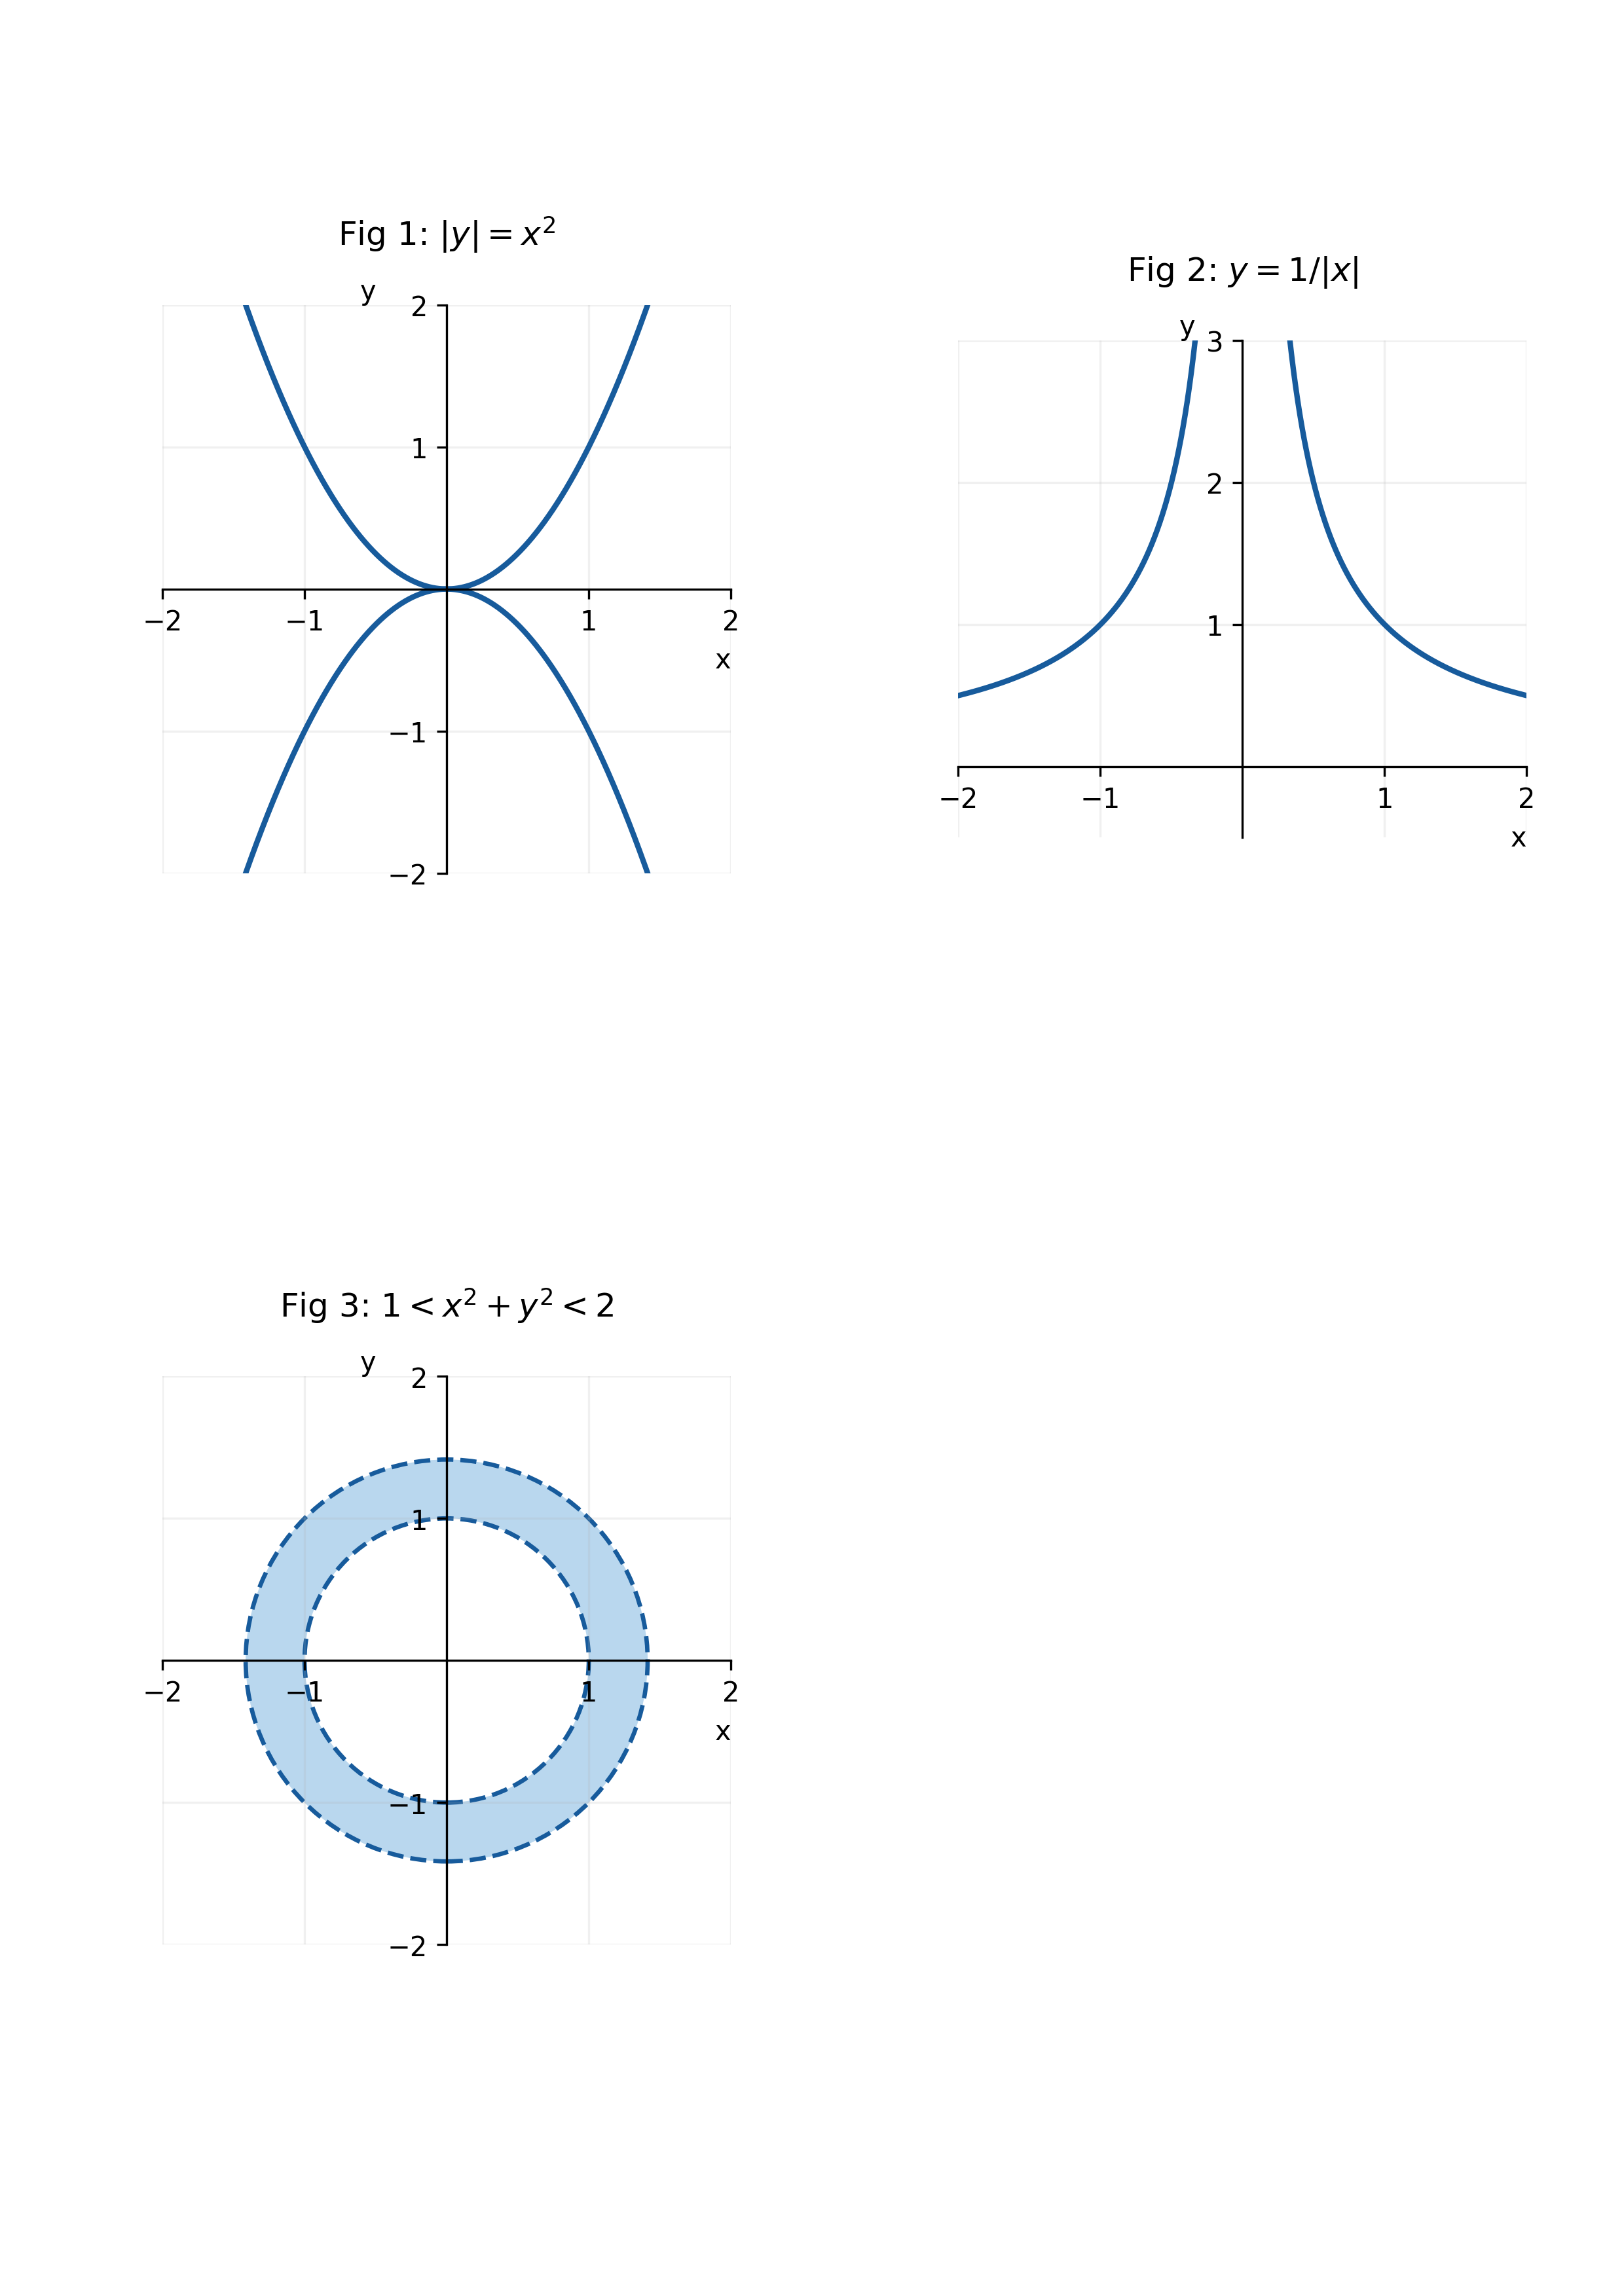
\includegraphics[width=0.5\textwidth,height=0.5\textheight,keepaspectratio]{Diagrams/Topology_WK_3_Q3.png}
\end{center}

\newpage
\noindent
I hope it is OK to use mainly descriptive solutions for this problem.\\
\\
(i) This set is path connected - hence connected!\\
\\
(ii) I assume that we are excluding the point where $x=0$. Here we can split $R^2$ into
two (open) half-planes (either side of $x=0$).  They don't overlap and they contain the complete set.\\
\\
(iii) The annulus when intersected with open sets of $R^2$ give connected sets of the annulus.\\
Hence, the annulus is also connected.\\
\\
(iv) Take $S= \mathbb{R} \setminus \mathbb{Q}$.  Then consider the two sets in $S$ defined by:\\
$U_1 = (-\infty, 1) \cap S$ and $U_2 = (1, \infty) \cap S$ - part of the induced topology.\\
\\
It is clear that: $U_1, U_2$ are both not empty, $U_1 \cap U_2 = \emptyset$ and
that $S=U_1 \cup U_2$.  We therefore conclude that $S=\mathbb{R} \setminus \mathbb{Q}$ is NOT connected.

\newpage
\section*{Exercise 4}
\begin{enumerate}
\item[a)] Let $(X,\mathcal{U})$ be a connected topological space. Show that the only clopen (both closed and open) sets in $X$ are $\varnothing$ and $X$.
\item[b)] Let $X$ be any set. Find the connected subsets of $(X,\mathcal{U})$ in each of the following cases:
\begin{enumerate}
\item[i)] $\mathcal{U}=\{\varnothing,X\}$ is the trivial topology;
\item[ii)] $\mathcal{U}=\mathcal{P}(X)$ is the discrete topology.
\end{enumerate}
\end{enumerate}
\noindent\textit{Note:} A subset $Y$ of $(X,\mathcal{U})$ is called connected if $(Y,\mathcal{U}_Y)$, with the induced topology, is a connected topological space.

\vspace{1cm}
\noindent
Answer:\\
(a) $(X,\mathcal{U})$ connected means $\nexists U,V\subset X$ (both open) s.t.
\begin{itemize}
\item $U\neq\varnothing\quad \text{ and } \quad V\neq\varnothing$
\item $U\cap V=\varnothing$
\item $U\cup V=X$.
\end{itemize}
Assume $\exists S\subset X$ which is ``clopen'' and $\emptyset \ne S \ne X$. Then
\begin{itemize}
\item $S$ is open
\item $X\setminus S$ is open (as $S$ is "clopen").
\item $S\cap(X\setminus S)=\varnothing$ - must hold by definition of complement.
\item $S\cup(X\setminus S)=X$ - must hold by definition of complement.
\end{itemize}
Contradiction. Hence, no such $S$ exists.\\
\\
(b) I will treat each topology in turn:
\begin{enumerate}
\item[(i)]
\begin{align*}
\mathcal{U} & = \{\varnothing,X\}\\
\Rightarrow\quad\mathcal{U}_Y &= \{\varnothing,Y\}.
\end{align*}
It is not possible to find two open sets in $\mathcal{U}_Y$ s.t. $U\neq\varnothing,\ V\neq \varnothing$ with $U\cap V=\varnothing$\\
and $Y=U\cup V$. \\
\\
Hence: \underline{$Y$ is connected.}

\newpage
\noindent
\item[(ii)]
\begin{align*}
\mathcal{U} &= \mathcal{P}(X)\\
\Rightarrow\quad\mathcal{U}_Y &= \mathcal{P}(Y)
\end{align*}
The discrete topology is such that all sets are both open \& closed (i.e. clopen).\\
Using the result from part (i), we must conclude that:\\
\\
\underline{$Y$ is disconnected.}\\
\\
\textit{This only applies if $Y$ contains more than 1 point!!}
\end{enumerate}


\newpage
\section*{Exercise 5}
Let $(X,\mathcal{U})$ be a connected topological space. Prove that:
\begin{enumerate}
\item[i)] if $f:X\to\mathbb{Z}$ is continuous, where $\mathbb{Z}$ carries the discrete topology, then $f$ is constant;
\item[ii)] if $f:X\to\mathbb{Q}$ is continuous, where $\mathbb{Q}$ carries the topology induced by the Euclidean distance on $\mathbb{R}$, then $f$ is constant.
\end{enumerate}
\noindent Now consider a continuous function $h:[0,1]\to[0,1]$.
\begin{enumerate}
\item[iii)] Use part (i) to prove that $h$ has a fixed point.
\end{enumerate}
\noindent\textit{Hint:} For part (iii), you may want to consider the function
\begin{align*}
x\longmapsto\frac{h(x)-x}{|h(x)-x|}.
\end{align*}
Where is it well-defined? Is it continuous?

\vspace{1cm}
\noindent
Answer:\\
\\
(i) $(X, \mathcal{U})$ is a topological space which is connected and 
$f:X\to\mathbb{Z}$ continuous with $\mathbb{Z}$ having the discrete topology.\\
\\
Then, for every $z\in\mathbb{Z}$, we have that $\{z\}$ is an open set (with the discrete topology) and
as $f$ is continuous: $f^{-1}(\{z\})$ is open in $X$.  Consequently, for any $T \subset \mathbb{Z}$:
\begin{align*}
f^{-1}(T) \in \mathcal{U}
\end{align*}
Now let $f$ take at least two distinct values on $\mathbb{Z}$. Let one such value be $k$.\\
Then, let $U=\{k\}$ - clearly $U$ is open in $\mathbb{Z}$.\\ 
Also let $V=\{z\in\mathbb{Z}\mid z \ne k\}$ - also clearly open in $\mathbb{Z}$.\\
Then:
\begin{align*}
f^{-1}(U)&=\bar{U}\quad\text{is open in }X.\\
f^{-1}(V)&=\bar{V}\quad\text{is open in }X.
\end{align*}
Obviously:
\begin{align*}
\bar{U}&\neq\varnothing\quad\&\quad\bar{V}\neq\varnothing.\\
\bar{U}\cap\bar{V}&=\varnothing\\
\text{and}\quad U\cup V&=X.
\end{align*}
Contradiction, as this means that $X$ is not connected. Hence, it is not possible for $f$ to be non-constant.\\
\qed

\newpage
\noindent
(ii) Assume $f:X\to\mathbb{Q}$ is \underline{not} constant. Then $\exists x_1,x_2\in X$ s.t. $f(x_1)=q_1,\ f(x_2)=q_2$ where $q_1,q_2\in\mathbb{Q}$
and $q_1\neq q_2$.\\
\\
Assume $q_1<q_2$. Take any irrational number between $q_1$ \& $q_2$ -- e.g.
\begin{align*}
i=q_1+\frac{1}{\sqrt{2}}(q_2-q_1)
\end{align*}
Then $O_1=(-\infty,i)$ \& $O_2=(i,\infty)$ are both open in $\mathbb{R}$
\begin{align*}
\Rightarrow\quad O_1\cap\mathbb{Q}=R_1\quad\&\quad O_2\cap\mathbb{Q}=R_2
\end{align*}
are both open in $\mathbb{Q}$ (with its induced topology).\\
\\
As $f$ is continuous $f^{-1}(R_1)$ \& $f^{-1}(R_2)$ are both open in $X$, both are non-empty.\\
Now, as $R_1\cup R_2=\mathbb{Q}$
\begin{align*}
f^{-1}(\mathbb{Q}) &= X \\
  &= f^{-1}(R_1\cup R_2) \\
  &= f^{-1}(R_1)\cup f^{-1}(R_2) \tag{5.1}
\end{align*}
Also: $R_1\cap R_2 = \varnothing$ and hence:
\begin{align*}
f^{-1}(R_1\cap R_2) &= f^{-1}(R_1)\cap f^{-1}(R_2) \\
&= f^{-1}(\emptyset) \\
&= \varnothing.
\end{align*}
The two open and non-empty sets $f^{-1}(R_1)$ \& $f^{-1}(R_2)$ suffice to show that $X$ is \textbf{not} connected.\\
\\
Contradiction!  Hence, f MUST be constant.\\
\\
(iii) We are given a continuous function $h:[0,1]\to[0,1]$\\
we define a new function:
\begin{align*}
f(x)=\frac{h(x)-x}{|h(x)-x|}
\end{align*}
If we assume that $h$ has no fixed pt in $[0,1]$ then $f$ is always well defined and continuous on $[0,1]$ taking values of $\pm1$.\\
Hence
\begin{align*}
f:[0,1]\to\{-1,+1\}\quad(\subset\mathbb{Z}).
\end{align*}
$\{-1,+1\}$ has the discrete topology (obtained when we intersect this set with the Euclidean topology defined on $\mathbb{R}$).\\
We know that under the Euclidean topology the set $[0, 1]$ is connected.
The codomain of $f$ is a discrete topological space which means that the function MUST be constant if it is continuous.\\
\\
But this means that:
\begin{align*}
\frac{h(x)-x}{|h(x)-x|}\quad\text{is constant}\quad\forall x\in[0,1].
\end{align*}
But this clearly isn't true; since $f(0)=1; f(1)=-1$ must hold.\\
So, our assumption of no fixed points for $h$ is false. I.e.
\begin{align*}
\exists x\in[0,1]\quad\text{s.t.}\quad h(x)=x.
\end{align*}
\qed

\newpage
\section*{Exercise 6}
Let $(X,\mathcal{U})$ be a topological space. The space $X$ is called \textit{locally connected at $x\in X$} if every neighborhood of $x$ contains an open set $V$ with $x\in V$ such that $V$, equipped with the topology induced by $X$, is connected. The space $X$ is \textit{locally connected} if it is locally connected at every point. Replacing ``connected'' by ``path-connected'' gives the corresponding notions of \textit{locally path-connected at $x$} and \textit{locally path-connected}.
\begin{enumerate}
\item[a)] \textbf{The topologist's sine curve.} Let $S\subset\mathbb{R}^2$ have the induced topology and be defined by
\begin{align*}
S=\bigl(\{0\}\times[-1,1]\bigr)
\cup\{(x,\sin(1/x)):x\in(0,1]\}.
\end{align*}
Show that $S$ is connected but not locally connected.
\item[b)] \textbf{The topologist's comb.} Let $C\subset\mathbb{R}^2$ have the induced topology and be defined by
\begin{align*}
C=\bigl(\{0\}\times[0,1]\bigr)
\cup\bigl([0,1]\times\{0\}\bigr)
\cup\bigcup_{n\in\mathbb{N}}\bigl(\{1/n\}\times[0,1]\bigr).
\end{align*}
Show that $C$ is path-connected but not locally path-connected.
\end{enumerate}


\end{document}
